\documentclass{beamer}
% \documentclass[handout,xcolor=pdftex,dvipsnames,table]{beamer}

\mode<presentation>
{
  \usetheme{Warsaw}
  \usecolortheme{whale}
  % or ...

  \setbeamercovered{transparent}
  % or whatever (possibly just delete it)
  \setbeamertemplate{navigation symbols}{}
}

\setbeamertemplate{itemize items}[ball]
\setbeamertemplate{itemize subitem}[triangle]
\setbeamertemplate{itemize subsubitem}[circle]
\setbeamercovered{transparent}

\usepackage{palatino} 
\usepackage{listings} % Gives syntax highlighting for python code. 
\usepackage{color} % Used for syntax highlighting. 
\usepackage{textcomp} % Used for syntax highlighting. 
\usepackage{caption}
\captionsetup{labelformat=empty,labelsep=none}
% This gives syntax highlighting in the python environment 
\definecolor{gray}{gray}{0.5} 
\definecolor{key}{rgb}{0,0.5,0} 
\lstset{
language=python,
basicstyle=\ttfamily\tiny, 
otherkeywords={1, 2, 3, 4, 5, 6, 7, 8 ,9 , 0, -, =, +, [, ], (, ), \{, \}, :, *, !}, 
keywordstyle=\color{blue}, 
stringstyle=\color{red},
showstringspaces=false,
alsoletter={1234567890},
otherkeywords={\ , \}, \{},
keywordstyle=\color{blue},
emph={access,and,break,class,continue,def,del,elif ,else,%
except,exec,finally,for,from,global,if,import,in,is,%
lambda,not,or,pass,print,raise,return,try,while},
emphstyle=\color{black}\bfseries,
emph={[2]True, False, None, self},
emphstyle=[2]\color{green},
emph={[3]from, import, as},
emphstyle=[3]\color{blue},
upquote=true,
morecomment=[s]{"""}{"""},
commentstyle=\color{gray}\slshape,
emph={[4]1, 2, 3, 4, 5, 6, 7, 8, 9, 0},
emphstyle=[4]\color{blue},
literate=*{:}{{\textcolor{blue}:}}{1}%
{=}{{\textcolor{blue}=}}{1}%
{-}{{\textcolor{blue}-}}{1}%
{+}{{\textcolor{blue}+}}{1}%
{*}{{\textcolor{blue}*}}{1}%
{!}{{\textcolor{blue}!}}{1}%
{(}{{\textcolor{blue}(}}{1}%
{)}{{\textcolor{blue})}}{1}%
{[}{{\textcolor{blue}[}}{1}%
{]}{{\textcolor{blue}]}}{1}%
{<}{{\textcolor{blue}<}}{1}%
{>}{{\textcolor{blue}>}}{1},%
numbers=none,
}

\newcommand{\putat}[3]{\begin{picture}(0,0)(0,0)\put(#1,#2){#3}\end{picture}}



\title[]{Python Workshop\\
Getting Started with Python}

\author[Fienen] % (optional, use only with lots of authors)
{Mike~Fienen}
\institute[USGS] % (optional, but mostly needed)
{
  U.S. Geological Survey\\
  Wisconsin Water Science Center, Middleton, Wisconsin USA
  }
  \titlegraphic{
\includegraphics[scale=0.5]{figures/c_USGSid1.pdf}}
  

\date[UQ12] % (optional, should be abbreviation of conference name)
{USGS National Groundwater Workshop, August 2012}

\subject{Python}


\begin{document}

\begin{frame}
  \titlepage
\end{frame}
\logo{\vspace{-0.3cm} 
\includegraphics[width=1.5cm]{figures/c_USGSid1.pdf}\hspace*{11.10cm}}  

\begin{frame}{Outline}
\tableofcontents
\end{frame}

\section{Preliminaries}
\begin{frame}[fragile]
\frametitle{What is Python?}
\begin{columns}
\column{.8\textwidth}
\begin{itemize}

\item{Python is a high-level, general programming language (relying much on C underneath) that is interpreted at run time through a command-line interface or scripting.} 
\pause
\item {Python is free, open-source, and (generally) platform-independent.}
\pause
\item {Python is built into many other programs and can wrap other languages like Java, C, FORTRAN, etc.}
\pause
\item{Python has a massive user community worldwide and growing within USGS.}
\end{itemize}
\column{.2\textwidth}
    \begin{figure}
    \putat{-40}{-60}{
        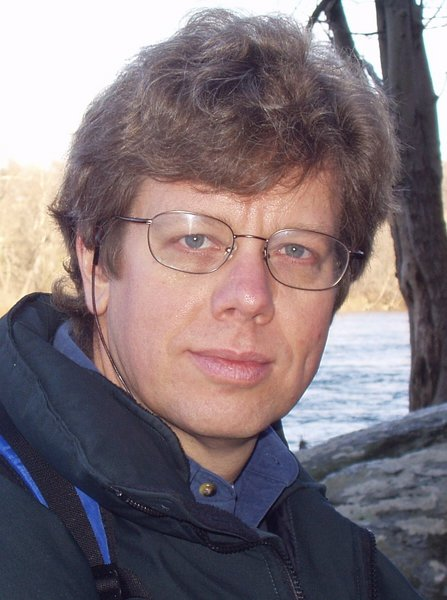
\includegraphics[width=2cm,height=2.68cm]{figures/Guido_van_Rossum.jpg}
	}
	\putat{-60}{-70}{Guido van Rossum}
	
       \putat{-55}{40}{
\includegraphics[width=3cm,height=.89cm]{figures/python.png}}
        
    \end{figure}       
\end{columns}

                  
\end{frame}

\begin{frame}[fragile]
\frametitle{Python Versions and Packages}
\begin{itemize}
\item{The two main version branches are 2.x and 3.x}
\item{We \emph{strongly} recommend sticking with 2.x \newline{}for now--Specifically \bf{2.7.3}}
\item{To do almost any substantial mathematics or statistics, you also need \texttt{numpy}}
\item{Basic 2-D graphics are possible using \texttt{matplotlib}}
\item{More advanced statistics are also available using \texttt{scipy}}
\item{Distributions already including many packages:}
\begin{itemize}
\item {pythonxy: for Windows only \url{http://pythonxy.com}
\includegraphics[scale=0.4]{figures/pythonxy.png}}
\item {EPD: Enthought Python Distribution for all Platforms \url{http://www.enthought.com}

\includegraphics[width=3cm,height=.86cm]{figures/enthought.png}}
\end{itemize}
\end{itemize}
\end{frame}

\begin{frame}[fragile]
\frametitle{Expanding Python with Packages}

Major capabilities (Numpy, Scipy, etc.) installed from a website using an installer (.msi, .exe, .dmg, .rpm)

For other packages, a couple options...
\begin{itemize}
\item Python Package Index \url{http://pypi.python.org}
\begin{itemize}
\item {For packages within PyPi, can use \texttt{easy\_install} at command line.}
\item {Packages at PyPi are installed using eggs. For more than you ever wanted to
 know about eggs, see \url{http://tinyurl.com/4jd5wud}}
\end{itemize}
\item Here's a blog post explaining for Win 7 \url{http://tinyurl.com/7hf9ml6}
\end{itemize}
\end{frame}

\section {Resources}
\begin{frame}[fragile]
\frametitle{Getting Help: Active and Helpful Python Community}
\begin{itemize}
\item Stackoverflow \url{http://stackoverflow.com}
\pause
\item A Useful Glossary \url{http://docs.python.org/glossary.html#glossary}
\pause
\item Python Official Docs \url{http://www.python.org/doc/}
\item Numpy and Scipy Official Docs \url{http://docs.scipy.org/doc/}
\pause
\item Numpy and Scipy Cookbook \url{http://www.scipy.org/Cookbook/}
\pause
\item Matplotlib \url{http://matplotlib.sourceforge.net/index.html}
\item Matplotlib Gallery (ridiculously cool) \url{http://matplotlib.sourceforge.net/gallery.html}
\pause
\item If you already known some MATLAB \url{http://www.scipy.org/NumPy_for_Matlab_Users/}
\end{itemize}
\end{frame}
%%%
% COMMAND LINE STUFF
%%%

\begin{frame}[fragile]
\frametitle{Command Line: Launch and Enter Commands}

Type ``python" to launch python
\begin{lstlisting}
c:\>python
Enthought Python Distribution (EPD) free version -- www.enthought.com
Version: 7.1-1 (32-bit)
(type 'upgrade' or see www.enthought.com/epd/upgrade to get the full EPD)

Python 2.7.2 |EPD_free 7.1-1 (32-bit)| (default, Jul  3 2011, 15:40:35) 
[GCC 4.0.1 (Apple Inc. build 5493)] on darwin
Type "packages", "demo", "upgrade" or "enthought" for more information.
>>>
>>>print 'hello world'
hello world
\end{lstlisting}
\pause
All commands that result in output display it on the screen
\begin{lstlisting}
>>> a=['this','is','a','list']
>>> a
['this', 'is', 'a', 'list']
>>> a[0]
'this'
\end{lstlisting}

\end{frame}

%%%
% MODULES/PACKAGES
\section{Modules and Packages}
\begin{frame}[fragile]
\frametitle{Packages, Modules, Namespaces}
First, a couple definitions.
\begin{description}
\item[Script:] A text file containing variables, functions, and definitions that can be 
 loaded for use at command line or in another script
\item[Module:] A script containing definitions for a specific purpose
\item[Package:] A group of modules
\item[Namespace:] A base name for a module used to organize and keep track of its provenance.
\end{description}
\end{frame}

\begin{frame}[fragile]
\frametitle{Packages, Modules, Namespaces at Command Line}
There are several ways to import a module or package.
\begin{itemize}
\pause
\item Preserving the namespace as the module name
\begin{lstlisting}
import numpy
\end{lstlisting}
To use the function \texttt{sqrt} must type
\begin{lstlisting}
s9 = numpy.sqrt(9)
\end{lstlisting}
\pause
\item {You can also provide an alias...}
\begin{columns}[c]
\column{3.5cm}
...for the namespace
\begin{lstlisting}
import numpy as np
s9 = np.sqrt(9)
\end{lstlisting}
\column{4.5cm}
...or for the function
\begin{lstlisting}
from numpy import sqrt as pow_to_minus_pfive
s9 = pow_to_minus_pfive(9)
\end{lstlisting}
\end{columns}
\pause
\item Or import the function without the namespace \emph{(danger!)}
\begin{lstlisting}
from numpy import *
s9 = sqrt(9)
\end{lstlisting}
\end{itemize}
\end{frame}

\begin{frame}[fragile]
\frametitle{Module Example}

\begin{lstlisting}
import antigravity
import this
\end{lstlisting}

\end{frame}

\section{Scripts}
\begin{frame}[fragile]
\frametitle{Using Scripts}
Scripts allow you to save the logic and definitions of a program much in the
 way compiled source code does for FORTRAN, C, and other languages.
 \newline{}
 \newline{}
The basic idea is to contain all code, in the same way you would type it into an interactive 
command window, in a file with the extension \texttt{.py}
\newline{}
\newline{}
You can then execute the script by typing \newline{} \texttt{python <scriptname>.py} \newline{}at the command line.
\end{frame}

\begin{frame}[fragile]
\frametitle{Using Scripts: An Example}

\end{frame}




\end{document}